\chapter{Architecture}
\label{sec:architecture}
\minitoc
\vspace*{1cm}

This chapter illustrates the general design of the fuzzer without going into too much technical detail. The in-depth breakdown of the fuzzer's components is thoroughly described in Chapter ~\ref{sec:implementation}. The key components elaborated on in this chapter are the high-level working view of \pname{}, the mutations made to the requests, and the different vulnerabilities in web applications that \pname{} is designed to detect.

\section{A Fuzzing Session}
\pname{} constitutes two intertwined components that work together in providing a guided fuzzing approach to find web application vulnerabilities. The first
component is the instrumentation of the target web application, that provides feedback to the fuzzer on which basic blocks were visited so as to deduce if new control paths have been discovered. For the instrumentation process, \pname{} adopts similar techniques to how AFL instruments binaries but in our case we adapted them to work in web applications. 

The second component is the fuzzing application with all its core functionalities responsible for sending requests from a dynamic request queue, reading their respective responses, parsing them to provide an informed decision on what the next request should be and displaying various statistics about the fuzzing session to the user. The fuzzer also features an inbuilt crawler that scans the HTML responses to detect anchor and form elements that can provide new, unseen paths of the web application to further explore.

A regular fuzzing session using \pname{} can be seen in Figure ~\ref{fig:architecture}. It displays the process from the point the request is sent, up to the stage where a response is received. A request can be produced in one of two ways; it can be in a mutated form of a previously made request which turned out to be interesting or as a new link that has been discovered by the inbuilt crawler but has not been visited yet. When the response is received, it is parsed in order to extract the execution time, vulnerabilities it may have triggered, coverage score, and to record newly discovered links.

\begin{figure}[ht]
 \centering
 \captionsetup{justification=centering}
 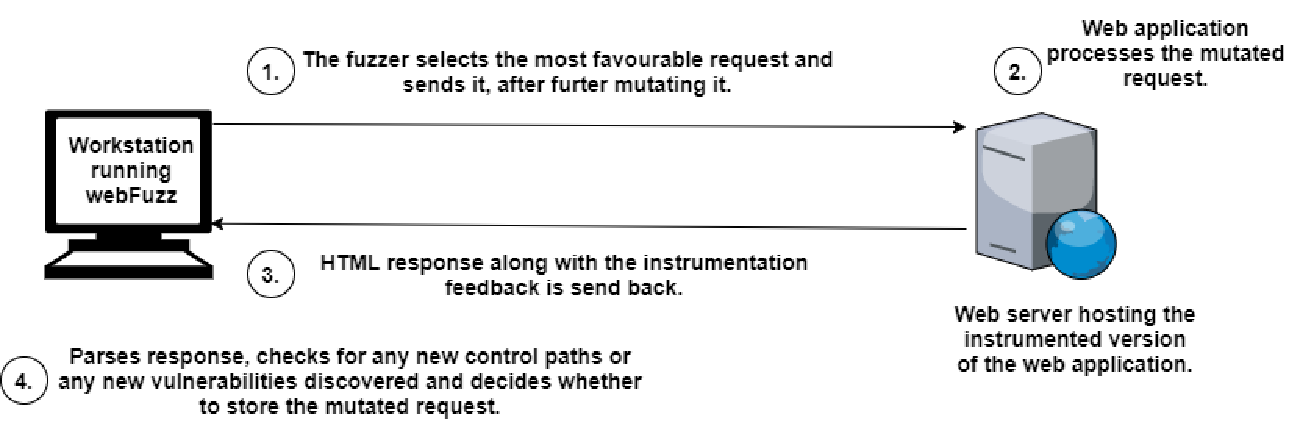
\includegraphics[width=\linewidth]{figures/architecture.pdf}
 \caption{\textit{High-level overview of a \pname{} fuzzing session}}
 \label{fig:architecture}
\end{figure}

\section{Mutations}
In most cases, sending randomly generated inputs will be quickly rejected by the target program as the data is syntactically invalid. One way to increase our chances of obtaining valid input is through mutational fuzzing where small modifications are made to existing inputs that may still keep the input valid, yet exercise new behaviour. Mutation-based fuzzers such as EFS ~\cite{efs2007} and AFL ~\cite{zalewski2015american} actively see the code paths executed on the target for each input they send and make adjustments accordingly. 

For creating fuzz test cases, mutation is a core part of the fuzzing process. It is vital because we need it to maintain diversity in our test cases to avoid stagnation on a suboptimal plateau in the search space ~\cite{seal2016Genetic}. Choosing which mutation function to use to detect the most vulnerabilities, is both a challenging and empirical task. 

If changes made to the input are too conservative, only limited code coverage will be achieved as there may not be enough to trigger new control flows whereas over-aggressive tweaks can destroy much of the input data structure and lead to the test cases failing at a premature stage of the execution ~\cite{zalewski2014Mutations}.

\pname{} currently supports five kinds of mutation functions, although the tool can be easily
extended to support custom GET or POST parameter mutations. The mutation functions employed are; injection of known XSS payloads, mixing the parameters from other requests (cross-over), insertion of a randomly generated payload, insertion of syntax aware payloads and altering the
parameter types. Some parameters may get randomly opted out from the mutation process. 

This can be useful in cases where certain parameters need to remain unchanged for designated areas of the program to execute. Unlike many fuzzers that employ malicious payload generation via the use of genetic algorithms, guided by an attack grammar ~\cite{duchene2014kameleonfuzz}, \pname{} chooses randomly from a corpus that consists of real-life known XSS payloads. The corpus was created with payloads that were found scattered across the internet, mainly in open-source repositories ~\cite{seclist,xsspayloadfirst,xsspayloadsecond}.

A small sample of XSS payloads contained in the corpus can be viewed in Table ~\ref{xss_payload_tables}. Such payloads can further mutate by prepending or appending to them random strings or specific HTML, JavaScript and PHP syntax tokens. Generating payloads from scratch using complex algorithms may have zero false positives but it is, nevertheless, time consuming.

\begin{table}[ht]
\centering
 \begin{tabular}{@{}|l|l|@{}}
 \hline
 \textbf{ } & \textbf{Corpus of known Cross-Site Scripting payloads} \\ 
 \hline\hline
 1 & <form onsubmit=alert(1)><input type=submit> \\ 
 \hline
 2 & <a draggable="true" ondragstart="alert(1)">test</a> \\ 
 \hline
 3 & <abbr id=x tabindex=1 onbeforedeactivate=alert(1)></abbr><input autofocus> \\ 
 \hline
 4 & <body onscroll=alert(1)><div style=height:1000px></div><div id=x></div> \\ 
 \hline
 5 & <canvas onbeforepaste="alert(1)" contenteditable>test</canvas> \\
 \hline
 6 & <nav onmouseover="alert(1)">test</nav> \\
 \hline
 7 & <style onreadystatechange=alert(1)></style> \\
 \hline
 \textbf{...} & \textbf{.....} \\
 \hline
 \end{tabular}
 \captionsetup{justification=centering}
 \caption[Cross-Site Scripting payloads corpus]{\textit{Randomly selected XSS payloads from the corpus \pname{} uses during a fuzzing session. The corpus consists of thousands of payloads}}
 \label{xss_payload_tables}
\end{table}

Although arrays in URL strings are not clearly defined in RFCs and their format is more framework specific, some web applications rely on them or are oblivious to their existence. Therefore, an input type altering mutation was added, where an input parameter that is
expected to be parsed as a string in the web application is transformed into an array or vice versa. Web applications not equipped to process unexpected types of input can be prone to glitches and bugs.

Using evolutionary algorithms in the test case creation process is widely practised in fuzzers
to optimize solution searching ~\cite{seal2016Genetic}, \pname{} will also mix GET or POST parameters from various favourable requests to generate new inputs. Contrary to how evolutionary algorithms work, this crossing over of input is not defined as a necessary step in each new input creation but can happen with a medium probability.

\section{Detecting Vulnerabilities}
\pname{} is able to detect Reflected and Stored Cross-Site Scripting(XSS) vulnerabilities, and subsequently, web applications that can be exploited for Distributed Denial of Service (DDoS) attacks. To detect such vulnerabilities, we conducted a string-matching process for the injected, possibly malicious, payload in the returned HTML response. This method is more efficient in terms of speed, however, it can result in a high ratio of false positives, as the location of the payload in the response is not accounted for. 

False positives arise when the tool reports that an XSS was detected when in fact there is none. One example is when the XSS payload is returned enclosed with double quotes inside an HTML element's attribute. If the web application correctly escapes any double quotes found in the XSS payload then the payload will not be executable. There are plans to improve the efficiency of our XSS detection method which is discussed in Chapter ~\ref{sec:discussion}.
